\section{Simulation}
Simulations are conducted in the Gazebo simulator within the ROS environment. UAV used in experiments is the $\mu$Morus which can be found in the \textit{mmuav\_gazebo} repository \cite{gitLink}, along with its model parameters. Two experiments will be conducted with different methods of CoG variation: 
\begin{itemize}
	\item UAV control based on moving masses
	\item UAV control based on payload carried by manipulator arms
\end{itemize}
Control parameters for the first case are chosen as follows:
\begin{equation*}
	\text{k}_x = 
	\begin{bmatrix}
		10 &  0  &  0 \\
		 0 & 10  &	0 \\ 
		 0 &  0  & 50 	
	\end{bmatrix}
	\, , \,	
	\text{k}_v =
	\begin{bmatrix}
		3.75 & 0 & 0 \\
		0 & 3.75 & 0 \\
		0 & 0 & 20
	\end{bmatrix}
\end{equation*}
\begin{equation*}
	\text{k}_R = 
	\begin{bmatrix}
		1.5 & 0 & 0 \\
		0 & 1.5 & 0 \\
		0 & 0 & 10
	\end{bmatrix}
	\, , \,
	\text{k}_\Omega = 
	\begin{bmatrix}
		0.65 & 0 & 0 \\
		0 & 0.65 & 0 \\
		0 & 0 & 1.54
	\end{bmatrix}
\end{equation*}

\noindent Rotational control parameters, in the second case, stay the same, while translational parameters are the following: 
\begin{equation*}
	\text{k}_x = 
	\begin{bmatrix}
		6 &  0  &  0 \\
		0 & 6  &	0 \\ 
		0 &  0  & 50 	
	\end{bmatrix}
	\, , \,	
	\text{k}_v =
	\begin{bmatrix}
		2.5 & 0 & 0 \\
		0 & 2.5 & 0 \\
		0 & 0 & 20
	\end{bmatrix}
\end{equation*}
For both cases, initial parameters are obtained by considering the error dynamics \ref{error_dynamics_linear} and \ref{error_dynamics_angular} in the equilibrium state. However, they are further tuned for better performance.\\
It is important to note that the actuator dynamics of moving masses and manipulators is taken in consideration within the Gazebo simulation environment. Furthermore there is a slight transient delay when increasing or decreasing rotor velocity which results in a non-instantaneous control force change. \\
\indent The chosen trajectory tracking problem is formulated as a rotating spiral:
\begin{gather*}
	\textbf{x}_d(t) = [0.4\text{t}; \, 0.5\text{sin}(\pi\text{t}); \, 0.6\text{cos}(\pi\text{t}) + 2] \\
	\textbf{b}_{1,d}(t) = [\text{cos}\left(\frac{\pi}{5}\text{t}\right); \, \text{sin}\left(\frac{\pi}{5}\text{t}\right); \, 0]
\end{gather*}
\noindent In the first case the total trajectory time is 20s while in the second case it will last 30s. Initial position and orientation is chosen at the start of the trajectory. \\
\todo[inline]{Simulirati sa masama.}
\begin{figure}[h!]
	\centering
	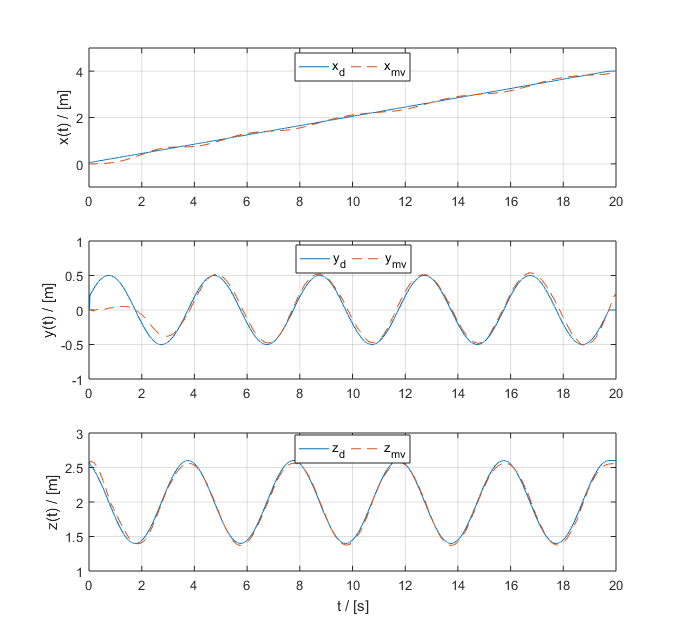
\includegraphics[width=\columnwidth]{./pictures/mmc_traj_pos.png}
	\caption{Comparison of the desired $\textbf{x}_d$ and measured position values $\textbf{x}_{mv}$. (Using the moving mass control concept.)}
	\label{fig:traj_pos}
\end{figure}

\begin{figure}[h!]
	\centering
	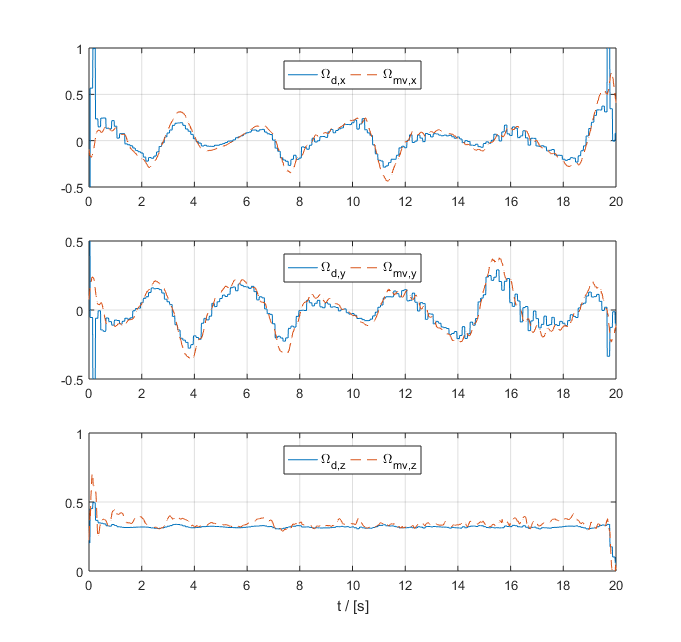
\includegraphics[width=\columnwidth]{./pictures/mmc_traj_omega.png}
	\caption{Comparison of desired $\mb{\Omega}_d$ and measured $\mb{\Omega}_{mv}$ angular velocity values. (Using the moving mass control concept.)}
	\label{fig:traj_omega}
\end{figure}

\begin{figure}
	\centering
	\begin{minipage}{0.5\columnwidth}
		\centering
		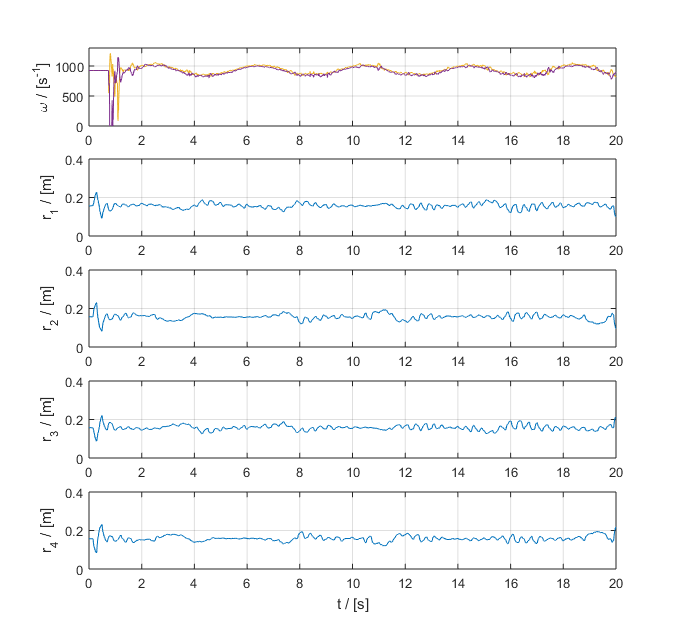
\includegraphics[width=\columnwidth]{./pictures/mmc_traj_rotorVel_massOff.png}
		\caption*{a)}
		\label{fig:rotorVel_massOff}
	\end{minipage}%
	\begin{minipage}{0.5\columnwidth}
		\centering
		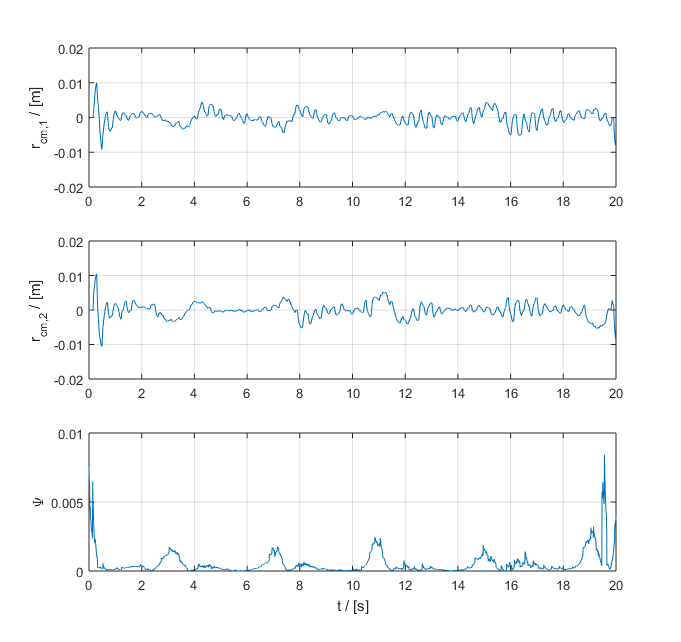
\includegraphics[width=\columnwidth]{./pictures/mmc_traj_rCm_attErr.png}
		\caption*{b)}
		\label{fig:rCm_attErr}
	\end{minipage}
	\caption{Control inputs are shown in figure a) in the following order: rotor velocities $\omega_i$ and mass offsets $r_i$. Figure b) shows first two components of CoG vector $\textbf{r}_{CoG}$ (third component is always zero since masses only move in x-y plane of the body-fixed frame) and attitude error function $\Psi$. (Using the moving mass control concept.)}
\end{figure}

\begin{figure}[h!]
	\centering
	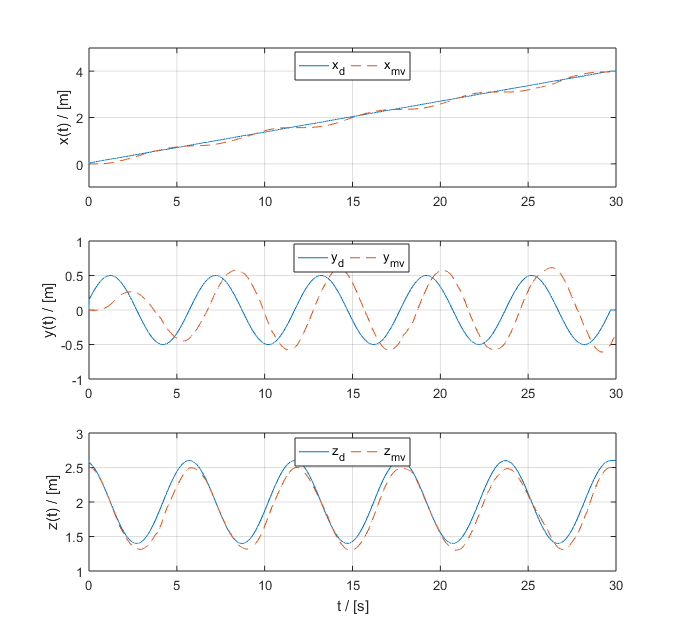
\includegraphics[width=\columnwidth]{./pictures/manip_traj_pos.png}
	\caption{Comparison of the desired $\textbf{x}_d$ and measured position values $\textbf{x}_{mv}$. (Using the manipulator control control.)}
	\label{fig:manip_pos}
\end{figure}

\begin{figure}[h!]
	\centering
	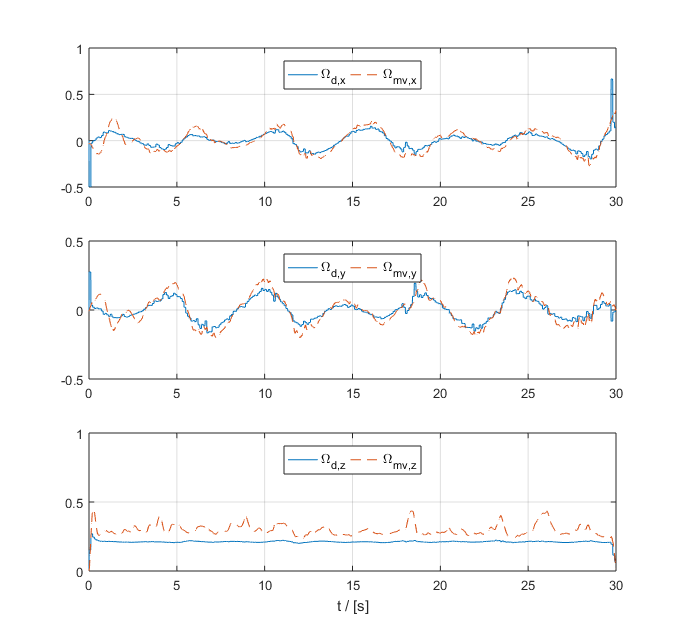
\includegraphics[width=\columnwidth]{./pictures/manip_traj_omega.png}
	\caption{Comparison of desired $\mb{\Omega}_d$ and measured $\mb{\Omega}_{mv}$ angular velocity values. (Using the manipulator control concept)}
	\label{fig:manip_omega}
\end{figure}
\begin{figure}[h!]
	\centering
	\begin{minipage}{0.5\columnwidth}
		\centering
		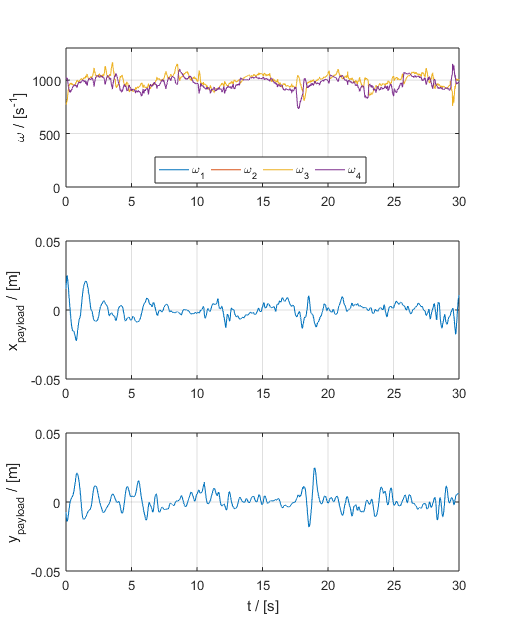
\includegraphics[width=\columnwidth]{./pictures/manip_traj_control.png}
		\caption*{a)}
		\label{fig:manip_control}
	\end{minipage}%
	\begin{minipage}{0.5\columnwidth}
		\centering
		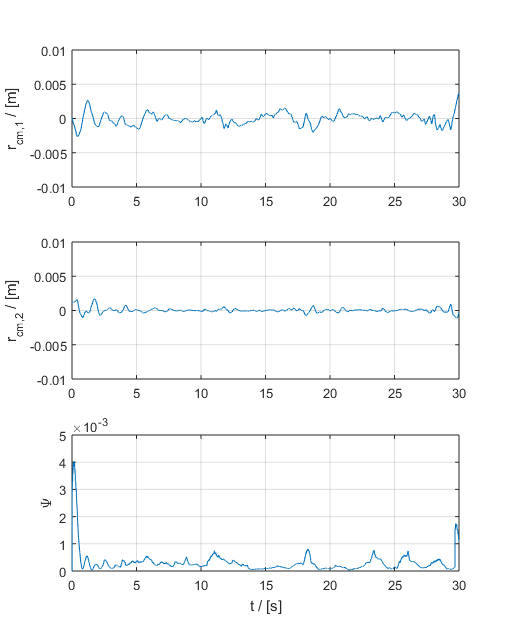
\includegraphics[width=\columnwidth]{./pictures/manip_traj_rcmPsi.png}
		\caption*{b)}
		\label{fig:manip_rcm}
	\end{minipage}
	\caption{Control inputs: rotor velocities $\omega_i$ and payload position; are shown in in figure a). Figure b) shows first two components of CoG vector $\textbf{r}_{CoG}$ and attitude error function $\Psi$.}
\end{figure}
